\documentclass[11pt]{memoir}

\usepackage{importationsprojet}

\pagestyle{empty}
\setlength{\parindent}{0pt}

\usepackage{ifthen}
\usepackage{multicol}
\usepackage{enumitem}

\newcounter{exercice}
\newcounter{question}
\newcounter{subpart}

\newcommand{\exercice}[1][Rien]
{
    \setcounter{question}{0}
    \setcounter{subpart}{0}
    \stepcounter{exercice}
    \par\noindent\underline{\textbf{Exercice \theexercice~:~%
    \ifthenelse{\equal{#1}{Rien}}%
    {}
    {%
    #1 points%
    }%
    }}%
}
\newcommand{\question}
{
    \setcounter{subpart}{0}
    \stepcounter{question}
    \par\textbf{\arabic{question})}
}
\newcommand{\subpart}
{
    \stepcounter{subpart}
    \par\textbf{\alph{subpart})}
}


\newlength{\hauteurRappels}
\newcommand{\rappels}[1]
{
    \settoheight{\hauteurRappels}{\hbox{#1}}
    \printlength{\hauteurRappels}
    \begin{center}
        \begin{tikzpicture}
            \draw (0,0) -- (0, \hauteurRappels) -- (\hauteurRappels, \hauteurRappels) -- (\hauteurRappels, 0) -- cycle;
        \end{tikzpicture}
    \end{center}
}

\newenvironment{questions}
{
    \setcounter{question}{0}
    \setcounter{part}{0}
    \setcounter{subpart}{0}
}
{

}

\newgeometry{margin=1.5cm}

\begin{document}
\begin{questions}

\exercice 

Décomposer les fractions suivantes en la somme d'un nombre entier et d'une fraction comprise entre 0 et 1.

\begin{multicols}{6}
\begin{enumerate}[label=\alph*)]
    \item $\dfrac{17}{8}$
    \item $\dfrac{24}{7}$
    \item $\dfrac{77}{3}$
    \item $\dfrac{83}{9}$
    \item $\dfrac{17}{4}$
    \item $\dfrac{27}{5}$
\end{enumerate}
\end{multicols}

\exercice 

Encadrer les fractions suivantes par deux entiers successifs.

\begin{multicols}{6}
\begin{enumerate}[label=\alph*)]
    \item $\dfrac{77}{8}$
    \item $\dfrac{83}{7}$
    \item $\dfrac{17}{3}$
    \item $\dfrac{24}{9}$
    \item $\dfrac{27}{4}$
    \item $\dfrac{17}{5}$
\end{enumerate}
\end{multicols}

\exercice 

Compléter le tableau suivant.

\begin{center}
\begin{tabular}{|c|c|c|c|c|c|}\hline
    Le nombre ci-dessous est divisible par & \phantom{aa}2\phantom{aa} & \phantom{aa}3\phantom{aa} & \phantom{aa}5\phantom{aa} & \phantom{aa}9\phantom{aa} & \phantom{aa}10\phantom{aa} \\\hline
    5912 & & & & & \\\hline
    34200 & & & & & \\ \hline
    54208 & & & & & \\ \hline
    317 & & & & & \\ \hline
    708 & & & & & \\ \hline
     & non & oui & non & non & non \\\hline
     & oui & oui & non & oui & non \\\hline
     & non & oui & oui & non & non \\\hline
     & oui & oui & oui & oui & oui \\\hline
     & non & non & non & non & non \\\hline
\end{tabular}
\end{center}

\exercice 

Sur le site de Météo France, il est possible de recueillir les données météorologiques liées à une ville, comme Crécy-la-Chapelle par exemple. \\
Intéressons-nous à la moyenne mensuelle des précipitations sur les données recueillies entre 1995 et 2010. \\(\textit{les données ont été arrondies au millimètre})

\begin{center}
\begin{tabular}{|l||*{12}{c|}}\hline
    Mois & jan. & fév. & mars & avril & mai & juin & juil. & août & sept. & oct. & nov. & déc. \\\hline
    Précipitations (\unit{\milli\meter}) & 52 &  & 50 & 50 & 59 &  & 66 & 69 & 49 &  & 61 & 62 \\\hline
\end{tabular}
\end{center}

\begin{center}
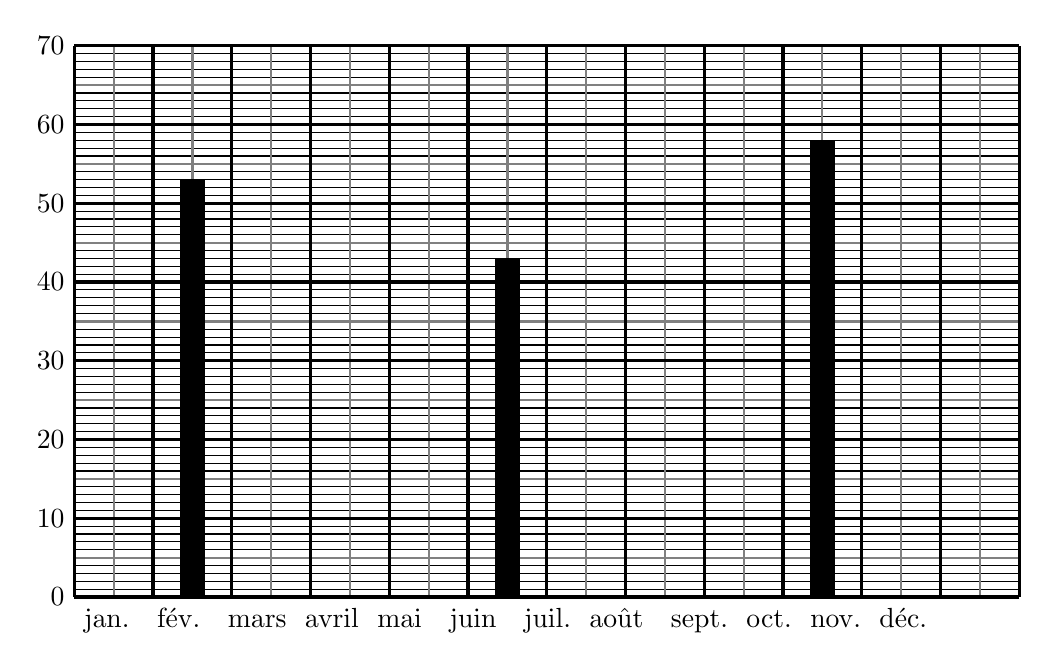
\begin{tikzpicture}
    \draw (0,0) grid[ystep=0.1] (12,7);
    \draw[gray, thick] (0,0) grid[step=0.5] (12,7);
    \draw[very thick] (0,0) grid[step=1] (12,7);
    \node[right] at (0,-0.3) {jan.~~~fév.~~~mars~~avril~~mai~~~juin~~~juil.~~août~~~sept.~~oct.~~nov.~~déc.};
    \foreach \x in {0,10,...,70} { \node[left] at (0,\x/10) {\x}; }
    \draw[fill=black] (5.35,0) rectangle (5.65,4.3);
    \draw[fill=black] (9.35,0) rectangle (9.65,5.8);
    \draw[fill=black] (1.35,0) rectangle (1.65,5.3);
\end{tikzpicture}
\end{center}

Compléter le tableau et le diagramme en barres, sachant qu'ils représentent le même jeu de données.

\end{questions}
\end{document}


